\section{Experiments}\label{sec:experiments}
We carried out a set of observations on the SV+ system. Firstly, we compared a SV+ program with the one in Verilog, to show the advantage of SV+ in describing reconfigurable structures. And then a cluster of implementations of AES algorithm generated from one copy of SV+ code were simulated, synthesized and mentioned.
\subsection{SV+ code \& Verilog}
%\begin{verbatim}
%%%%%%%%%%%%%%%%%%%%%%%%%%%%%%%%%%%%%%%%%%%%%%%%%%%%%%%
%module f2(in,out,s1,s0); module f3(in,out,s2,s1,s0);
%  ...(declares)            ...(declares)
%  wire[31:0] w1,w0;        wire[31:0] w2,w1,w0;
%                           wire[31:0] acc1,acc0;
%  assign out = w1 + w0;    assign out = acc1 + w0;
%  assign w1 = in << s1;    assign acc1 = w2 + w1;
%  assign w0 = in << s0;      	
%endmodule                  assign w2 = in << s2; 
%                           assign w1 = in << s1; 
%                           assign w0 = in << s0; 
%                         endmodule
%\end{verbatim}
%\vspace{3ex}
%\hrule
%\vspace{-2ex}
Here we discuss the code that compute equation\eqref{eq:code} in Verilog left side) and SV+.
\begin{equation}
out = in{<<}s3{+}in{<<}s2{+}in{<<}s1{+}in{<<}s0  
\label{eq:code}
\end{equation}
%\vspace{6ex}
%\hrule
%\vspace{-3ex}
\begin{verbatim}
Verilog:                     SV+
1. module scm(ports);     | module scm(ports);
2.   ...(declares)        |    ...(declares)
3.   reg[31:0] sum;       |    reg[31:0] sum;
4.   reg[31:0] tmp;       |    assign out = sum;
5.   always@(posedge clk) |    always@(posedge clk)
6.   if(rst_i)            |    if(rst_i)
7.      sum <= 0;         |      sum <= 0;
8.   else if(s_i3)        |    else if(fold_i)
9.      temp <= in << s3; |      fold(sum,in,s3,
10.  else if(s_i2)        |           s2,s1,s0);
11.     temp <= in << s2; | endmodule
12.  else if(s_i1)        |      
13.      tmp <= in << s1; |       
14.  else if(s_i0);       |  
15.     tmp <= in << s0;  |
16.  else if(add_i)       |
17.     sum <= sum + tmp; |
18. endmodule             | 
\end{verbatim}
%\vspace{-3ex}
We could recognize that:
%\vspace{-3ex}
\begin{itemize}
  \item[$\diamond$] In Verilog, designer needs to be careful to which $tmp$ should connect, in line 9 and 11.
  \item[$\diamond$] If we want to compute the shift-summation of more variables, for example $s3,s2,s1,s0$,sevral 
                    lines of boilerplate code should be added to the Verilog program. And for SV+ program, small 
                    changes to $fold(sum,in,$ $s5,s4,s3,s2,s1,s0)$ could do.
  \item[$\diamond$] Most important, if we want to use more resources to speed up the computation, rewriting on 
                    the 
                    Verilog is unavoidable, but SV+ code can remain unchanged. The compiler could see the  
                    trade-offs and do it.  
\end{itemize} 
%\subsection{Outputs from SV+ Compiler}
\subsection{Measure on Implementations of AES}
15 kinds of optimizations choices for AES are explored by SV+ system. The synthesis results of these implementations vary in architectures as well as in resource consuming and time cost. We synthesized these RTL descriptions in Synopsys using TSMC 0.18$um$ standard cell library. Table \ref{xxxx} shows the main measuring dimensions of these circuits. Where, configurations are the number of sbox (left most column) and mixcolumnx (top most line) sub-modules used in AES design. We could see that, configuration with the most modules has 2.5 times of gates number of that with fewest modules and 20\% of the cycles. Thus, the reconfigurations do make sense, since users can get considerable trade-offs between space and time. Table \ref{table:com} is about the comparison with other implementations. Ours provide many kinds of configurations which have different gates, and have high frequency.
%%%%%%%%%%%%%%%%%%%%%%%%%%%%%%%%%%%%%%%%%%%%%%%%%%%%%%%%%%%%%%%%%%%%%%%%%
\begin{table}[h]
\centering
\caption{Area and time cost of AES}
\subtable[Cycles]{
\begin{tabular}{|r|rrr|}\hline
 & \textit{1} & \textit{2} &  \textit{4} \\ \hline
\textit{1} & 218 & 200 & 191 \\ 
\textit{2} & 138 & 120 & 111 \\ 
\textit{4} & 98 & 80  & 71 \\ 
\textit{8} & 78 & 60  & 51\\ 
\textit{16}& 63 & 50  & 41 \\ \hline
\end{tabular}
}
\subtable[Gates]{
\begin{tabular}{|r|rrr|}\hline
 & \textit{1} & \textit{2} &  \textit{4} \\ \hline
 \textit{1}  & 6004 & 6314 & 6824 \\ 
 \textit{2}  & 6398 & 6742 & 7164 \\ 
 \textit{4}  & 7057 & 7350 & 7828 \\ 
 \textit{8}  & 8599 & 8875 & 9315 \\ 
\textit{16} & 11310& 11686 & 12069 \\ \hline
\end{tabular}
}
\label{xxxx}
\end{table}
\begin{table}[h]
\centering
\caption{Comparison with other AESs}
\begin{tabular}{|l|r|r|r|c|}\hline
Ref & Tech & Gates & Freq & Conf \\ \hline
\cite{Akashi:AES} & $0.18um$ & 7226 & $138_{MHz}$ &  \\ \cline{1-4}
\cite{Martin:AES} & $0.35um$ & 3595 & $100_{KHz}$ & 1\\ \cline{1-4}
%[6] & $0.25um$ & 12000 & $100_M$ & 1 \\ \cline{1-4}
\cite{Norbert:AES} & $0.6um$ & 8541 & $50_{MHz}$ & \\ \hline
\cite{Yibo:AES} & $0.18um$ & 6986 & $180_{MHz}$ & 3 \\ \hline
Ours & $0.18um$ & 6004,...,12069 & $180_{MHz}$ & 15 \\ \hline
\end{tabular}
\label{table:com}
\end{table} 
For silicon technology the area-time tradeoff has been nicely formalized by theorists as AT (area and time) bounds. Author in paper\cite{AT} shows that: 
\begin{equation}
AT^n = constant, \;\;\;n\; is\; between\; 1\; and\; 2
\label{eq:at}
\end{equation} 
Figure\ref{fig-mesure} is the two-dimension diagram between area-time of our AES implementations. The blue line is about gates and cycles of each implementation. And green line is function $xy=750000$. It reveals the area-time bounds approximately in keeping with \eqref{eq:at}, when $n=1$ and $constant = 750000$.
\begin{figure}[thbp]
\centering
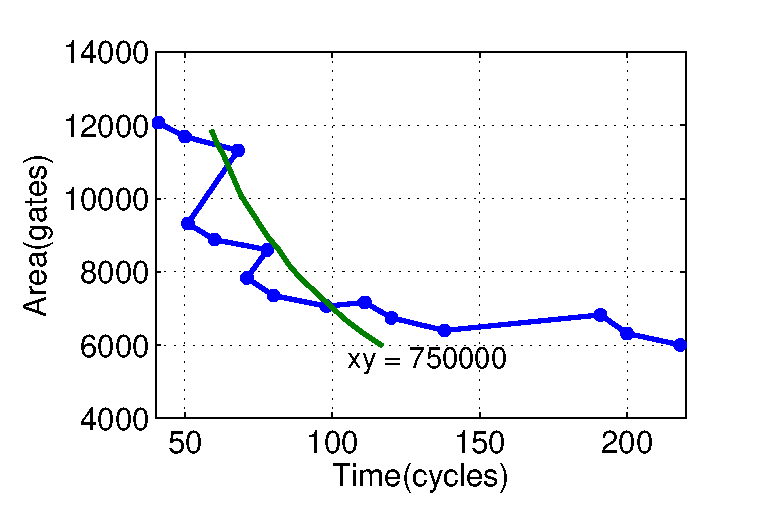
\epsfig{file=mesure4.eps,width=0.7\columnwidth}
\caption{Configurations and Resource cost of AES}
\label{fig-mesure}
\end{figure}
\subsection{Sythesis result of SCM, DCT and FFT}
In example SCM, there is a $fold$ re-configurable construct with 4 variables, so totally it has 3 different configurations. FFT has 3 $forloop$. Since each $forloop$ provides 3 optimization choices, FFT has as many as 27 kinds of configurations. DCT has also 3 $forloop$ and 36 kinds of implementations (Implementations of these three algorithm are in Appendix B).
Table \ref{table:confs} shows area and time cost of some configurations of these three algorithms.
%\vspace{-3ex}
\begin{table}[hb]
\centering
\caption{Some Confs. of SCM, FFT and DCT}
\begin{tabular}{|r|rr|r|rr|} \hline
\multicolumn{3}{|c|}{SCM} & \multicolumn{3}{c|}{DCT} \\ \hline
%DFT & & & FFT & & \\ \hline
\textit{conf.} & Gates & Cycles & \textit{conf.} & Gates & Cycles \\ \hline
\textit{1} & 1621 & 9 & \textit{1} & 4562 & 17 \\ 
\textit{2} & 2782 & 5 & \textit{2} & 4903 & 13 \\ 
\textit{3} & 4738 & 3 & \textit{3} & 5104 & 11 \\ \cline{1-3}
\multicolumn{3}{|c|}{FFT} & \textit{4} & 5208 & 10 \\ \cline{1-3}
\textit{conf.} & Gates & Cycles & \textit{5} & 4711 & 15 \\ \cline{1-3}
\textit{1} & 4562 & 13 & \textit{6} & 4806 & 14 \\
\textit{2} & 4923 & 11 & \textit{7} & 5298 & 8 \\
\textit{3} & 5133 & 10 & \textit{8} & 5362 & 7 \\
\textit{4} & 5427 & 8 & \textit{9} & 5503 & 5 \\
\textit{5} & 5540 & 7 & \textit{10} & 5642 & 4 \\
\textit{6} & 5761 & 5 & \textit{11} & 5419 & 6 \\
\textit{7} & 5902 & 4 & \textit{12} & 5179 & 9 \\ \hline
\end{tabular}
\label{table:confs}
\end{table}
Column $conf.$ is the serial number of configurations. Gates is the number of gate, Cycles is the number of cycle. They are all synthesized in frequency $180_{MHz}$.   
%%%%%%%%%%%%%%%%%%%%%%%%%%%%%%%%%%%%%%%%%%
